\documentclass{standalone}
\usepackage{tikz}
\usetikzlibrary{patterns, positioning}
\usepackage[sfdefault]{ClearSans} %% option 'sfdefault' activates Clear Sans as the default text font
\usepackage[T1]{fontenc}

\begin{document}
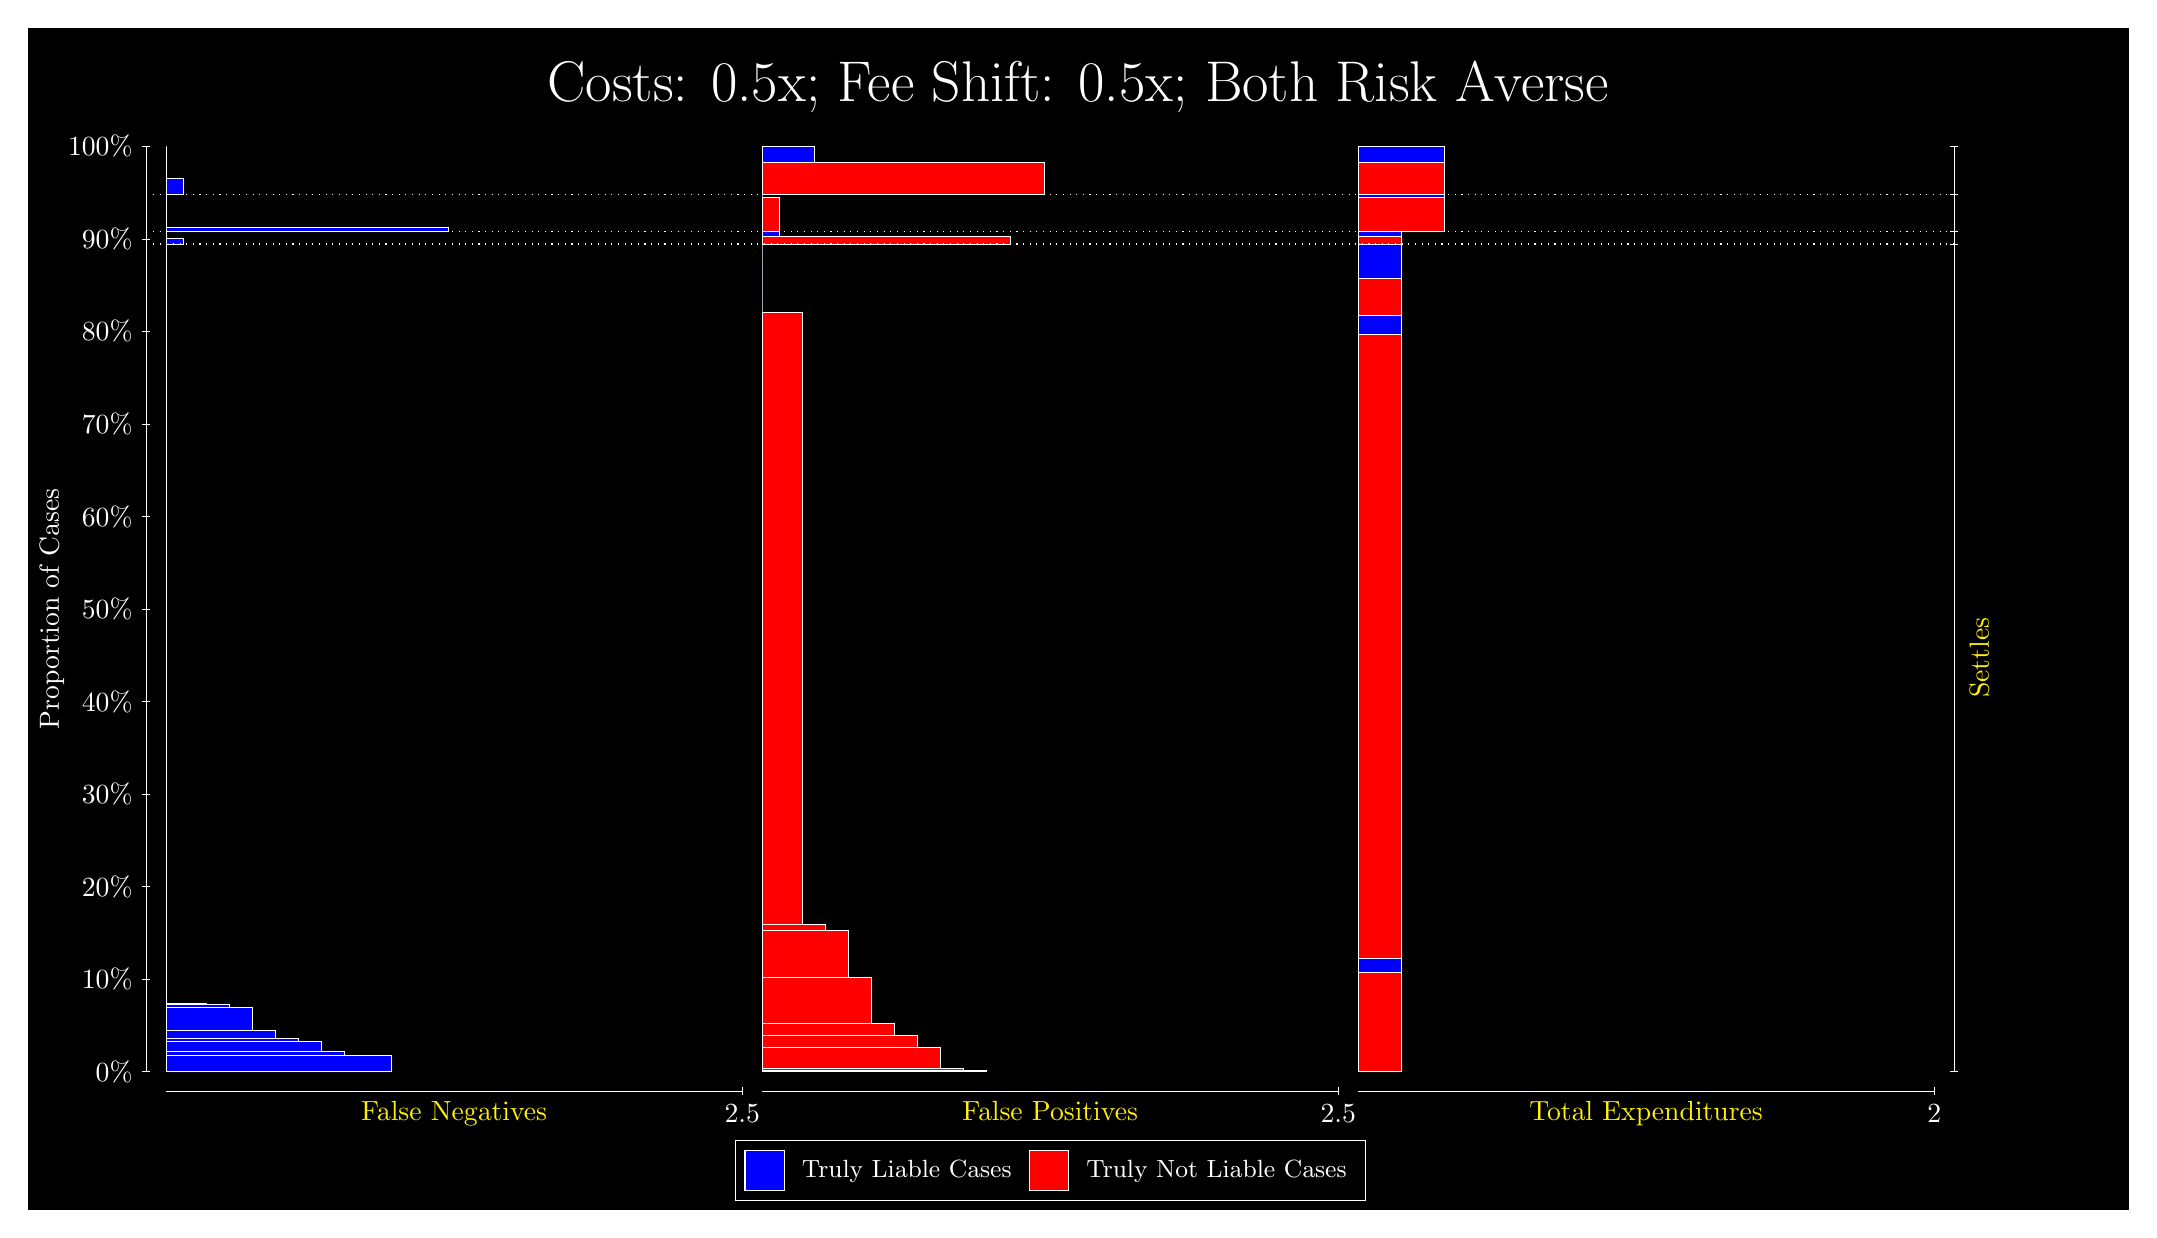
\begin{tikzpicture}
\draw[fill=black] (0,0) rectangle (26.667,15);
\draw[text=white] (0,13.5) rectangle (26.667,15) node[midway] {\huge Costs: 0.5x; Fee Shift: 0.5x; Both Risk Averse};
\draw[white, very thin] (1.5,1.75) -- (1.5,13.5);
\node[rotate=90, text=white, anchor=center] at (0.3, 7.625) {Proportion of Cases};
\draw[white, very thin] (1.45,1.75) -- (1.55,1.75);
\node[text=white, anchor=east] at (1.45, 1.75) {0\%};
\draw[white, very thin] (1.45,2.925) -- (1.55,2.925);
\node[text=white, anchor=east] at (1.45, 2.925) {10\%};
\draw[white, very thin] (1.45,4.1) -- (1.55,4.1);
\node[text=white, anchor=east] at (1.45, 4.1) {20\%};
\draw[white, very thin] (1.45,5.275) -- (1.55,5.275);
\node[text=white, anchor=east] at (1.45, 5.275) {30\%};
\draw[white, very thin] (1.45,6.45) -- (1.55,6.45);
\node[text=white, anchor=east] at (1.45, 6.45) {40\%};
\draw[white, very thin] (1.45,7.625) -- (1.55,7.625);
\node[text=white, anchor=east] at (1.45, 7.625) {50\%};
\draw[white, very thin] (1.45,8.8) -- (1.55,8.8);
\node[text=white, anchor=east] at (1.45, 8.8) {60\%};
\draw[white, very thin] (1.45,9.975) -- (1.55,9.975);
\node[text=white, anchor=east] at (1.45, 9.975) {70\%};
\draw[white, very thin] (1.45,11.15) -- (1.55,11.15);
\node[text=white, anchor=east] at (1.45, 11.15) {80\%};
\draw[white, very thin] (1.45,12.325) -- (1.55,12.325);
\node[text=white, anchor=east] at (1.45, 12.325) {90\%};
\draw[white, very thin] (1.45,13.5) -- (1.55,13.5);
\node[text=white, anchor=east] at (1.45, 13.5) {100\%};

\draw[white, very thin] (24.457,1.75) -- (24.457,13.5);
\draw[white, very thin] (24.407,1.75) -- (24.507,1.75);
\node[anchor=west] at (24.407, 1.75) {};
\draw[white, very thin] (24.407,12.26) -- (24.507,12.26);
\node[anchor=west] at (24.407, 12.26) {};
\draw[white, very thin] (24.407,12.423) -- (24.507,12.423);
\node[anchor=west] at (24.407, 12.423) {};
\draw[white, very thin] (24.407,12.893) -- (24.507,12.893);
\node[anchor=west] at (24.407, 12.893) {};
\draw[white, very thin] (24.407,13.5) -- (24.507,13.5);
\node[anchor=west] at (24.407, 13.5) {};

\draw[white, very thin, fill=blue] (1.75,1.75) rectangle (4.6044,1.9511);
\draw[white, very thin, fill=blue] (1.75,1.9511) rectangle (4.3116,1.9619);
\draw[white, very thin, fill=blue] (1.75,1.9619) rectangle (4.0188,2.0058);
\draw[white, very thin, fill=blue] (1.75,2.0058) rectangle (3.7261,2.1316);
\draw[white, very thin, fill=blue] (1.75,2.1316) rectangle (3.4333,2.1697);
\draw[white, very thin, fill=blue] (1.75,2.1697) rectangle (3.1406,2.2789);
\draw[white, very thin, fill=blue] (1.75,2.2789) rectangle (2.8478,2.5603);
\draw[white, very thin, fill=blue] (1.75,2.5603) rectangle (2.5551,2.6007);
\draw[white, very thin, fill=blue] (1.75,2.6007) rectangle (2.2623,2.6112);
\draw[white, very thin, fill=red] (1.75,2.6112) rectangle (1.75,12.26);
\draw[white, very thin, fill=blue] (1.75,12.26) rectangle (1.9696,12.328);
\draw[white, very thin, fill=red] (1.75,12.328) rectangle (1.75,12.423);
\draw[white, very thin, fill=blue] (1.75,12.423) rectangle (5.3362,12.467);
\draw[white, very thin, fill=red] (1.75,12.467) rectangle (1.75,12.893);
\draw[white, very thin, fill=blue] (1.75,12.893) rectangle (1.9696,13.095);
\draw[white, very thin, fill=red] (1.75,13.095) rectangle (1.75,13.5);
\draw[white, very thin, fill=red] (9.3189,1.75) rectangle (12.173,1.7607);
\draw[white, very thin, fill=red] (9.3189,1.7607) rectangle (11.88,1.7955);
\draw[white, very thin, fill=red] (9.3189,1.7955) rectangle (11.588,2.0575);
\draw[white, very thin, fill=red] (9.3189,2.0575) rectangle (11.295,2.2102);
\draw[white, very thin, fill=red] (9.3189,2.2102) rectangle (11.002,2.3626);
\draw[white, very thin, fill=red] (9.3189,2.3626) rectangle (10.709,2.9444);
\draw[white, very thin, fill=red] (9.3189,2.9444) rectangle (10.417,3.5422);
\draw[white, very thin, fill=red] (9.3189,3.5422) rectangle (10.124,3.6189);
\draw[white, very thin, fill=red] (9.3189,3.6189) rectangle (9.8312,11.398);
\draw[white, very thin, fill=blue] (9.3189,11.398) rectangle (9.3189,12.26);
\draw[white, very thin, fill=red] (9.3189,12.26) rectangle (12.466,12.355);
\draw[white, very thin, fill=blue] (9.3189,12.355) rectangle (9.5384,12.423);
\draw[white, very thin, fill=red] (9.3189,12.423) rectangle (9.5384,12.849);
\draw[white, very thin, fill=blue] (9.3189,12.849) rectangle (9.3189,12.893);
\draw[white, very thin, fill=red] (9.3189,12.893) rectangle (12.905,13.299);
\draw[white, very thin, fill=blue] (9.3189,13.299) rectangle (9.9776,13.5);
\draw[white, very thin, fill=red] (16.888,1.75) rectangle (17.437,3.0063);
\draw[white, very thin, fill=blue] (16.888,3.0063) rectangle (17.437,3.1868);
\draw[white, very thin, fill=red] (16.888,3.1868) rectangle (17.437,11.119);
\draw[white, very thin, fill=blue] (16.888,11.119) rectangle (17.437,11.358);
\draw[white, very thin, fill=red] (16.888,11.358) rectangle (17.437,11.818);
\draw[white, very thin, fill=blue] (16.888,11.818) rectangle (17.437,12.26);
\draw[white, very thin, fill=red] (16.888,12.26) rectangle (17.437,12.355);
\draw[white, very thin, fill=blue] (16.888,12.355) rectangle (17.437,12.423);
\draw[white, very thin, fill=red] (16.888,12.423) rectangle (17.986,12.849);
\draw[white, very thin, fill=blue] (16.888,12.849) rectangle (17.986,12.893);
\draw[white, very thin, fill=red] (16.888,12.893) rectangle (17.986,13.299);
\draw[white, very thin, fill=blue] (16.888,13.299) rectangle (17.986,13.5);
\draw[white, dotted] (1.5,12.26) -- (24.457,12.26);
\draw[white, dotted] (1.5,12.423) -- (24.457,12.423);
\draw[white, dotted] (1.5,12.893) -- (24.457,12.893);
\draw[white, very thin] (1.75,1.5) -- (9.0689,1.5);
\node[text=yellow, anchor=north] at (5.4094, 1.5) {False Negatives};
\draw[white, very thin] (9.0689,1.45) -- (9.0689,1.55);
\node[text=white, anchor=north] at (9.0689, 1.45) {2.5};

\draw[white, very thin] (9.3189,1.5) -- (16.638,1.5);
\node[text=yellow, anchor=north] at (12.978, 1.5) {False Positives};
\draw[white, very thin] (16.638,1.45) -- (16.638,1.55);
\node[text=white, anchor=north] at (16.638, 1.45) {2.5};

\draw[white, very thin] (16.888,1.5) -- (24.207,1.5);
\node[text=yellow, anchor=north] at (20.547, 1.5) {Total Expenditures};
\draw[white, very thin] (24.207,1.45) -- (24.207,1.55);
\node[text=white, anchor=north] at (24.207, 1.45) {2};

\node[text=yellow, centered, rotate=90] at (24.777, 7.0048) {Settles};




\draw (12.978300999999998,1.5) node[draw=none] (baseCoordinate) {};
\begin{scope}[align=center]
        \matrix[scale=0.5, draw=white, below=0.5cm of baseCoordinate, nodes={draw}, column sep=0.1cm]{
            \node[rectangle, draw, minimum width=0.5cm, minimum height=0.5cm, fill=blue] {}; &
            \node[draw=none, font=\small, text=white] (B) {Truly Liable Cases}; &
            \node[rectangle, draw, minimum width=0.5cm, minimum height=0.5cm, fill=red] {}; &
            \node[draw=none, font=\small, text=white] (B) {Truly Not Liable Cases}; \\
            };
\end{scope}

\end{tikzpicture}
\end{document}